\documentclass[10pt,french]{beamer}

% Theme selection
\usepackage{babel}
\usetheme{metropolis}
\usepackage{appendixnumberbeamer}
\usepackage{booktabs}
\usepackage[scale=2]{ccicons}
\usepackage{pgfplots}
\usepgfplotslibrary{dateplot}
\usepackage{xspace}
\usepackage{graphicx} 
\usepackage{url}

\usepackage{lmodern}

\newcommand{\themename}{\textbf{\textsc{metropolis}}\xspace}

\title{Projet 7Wonders}
\subtitle{Groupe A}
\date{\today}
\institute{Universit\'{e} C\^{o}te d'Azur}
\author{\textbf{Boutrik} Alexandre, \textbf{Diallo} Elhadj Oumar, \newline \textbf{Ghilane El Hassani} Abdelouarite, \textbf{Landoulsi} Aziz, \newline \textbf{Maniliuc} David, \textbf{Rahmouni} Mohamed Khalil}
\titlegraphic{\hfill
\includegraphics[height=2cm]{./logo_uni.png}}

\begin{document}

\maketitle

\begin{frame}{Table des matières}
  \setbeamertemplate{section in toc}[sections numbered]
  \tableofcontents[hideallsubsections]
\end{frame}

\section{Quelles fonctionnalités avons-nous réalisées ?}

\begin{frame}{Quelles fonctionnalités avons-nous réalisées ?}
    \begin{columns}
        \begin{column}{0.5\textwidth}
            \begin{itemize}
                \item Jeu complet avec \textit{toutes les mechaniques} implémentées dont le chaînage et les ressources à choix
                \item Intégralité des effets des cartes et des merveilles
                \item Configuration utilisateur en \texttt{toml}
                \item Modes d'exécution :
                  \begin{itemize}
                    \item \textbf{un} avec un déroulé visible et compréhensible (+log)
                    \item \textbf{plusieurs} pour un usage statistique
                  \end{itemize}
            \end{itemize}
        \end{column}
        \begin{column}{0.5\textwidth}
            \begin{itemize}
                \item Chargement des données de jeu a partir de fichiers \texttt{json}.
                \item Robots implémentés :
                  \begin{itemize}
                    \item 1 robot choisissant des cartes au \textit{hasard}
                    \item 4 robots \textit{spécialistes} se concentrant sur un seul but
                    \item 2 robots \textit{intelligents} choisissant les cartes en fonction du cours de la partie
                    \item 1 robot « \textit{meta} » se servant des stratégies spécialistes 
                  \end{itemize}
                \item 3 inflexions sur les 4 ont été implémentées
            \end{itemize}
        \end{column}
    \end{columns}
\end{frame}

\section{Quels grands choix de conception avons-nous faits ?}

 \begin{frame}{Conception clé : Structure du projet}
       \begin{block}{Architecture des modules :}
           Notre projet est structuré autour de plusieurs modules ayant claire :
           \begin{itemize}
               \item \textbf{models} : Contient les objets du domaine représentant l'état du jeu (joueurs, cartes, merveilles, etc.). 
                   %C'est le cœur de la structure du jeu.
               \item \textbf{core} : Abrite le \texttt{GameEngine}, le moteur principal qui orchestre le déroulement d'une partie.
               \item \textbf{ai} : Représente la logique et l'api des robots.
               \item \textbf{services} : Est garant de la contruction et du calcul de score.
               \item \textbf{io} : Gère les entrées/sorties, notamment l'affichage des informations pour l'utilisateur via \texttt{ConsoleReporter}.
               \item \textbf{stats} : Responsable de l'analyse des statistiques des parties jouées.
               \item \textbf{utils} : Fournit des fonctionnalités transverses comme la gestion de la configuration (\texttt{config.toml}) et la journalisation.
           \end{itemize}
       \end{block}
   \end{frame}

\begin{frame}{Conception clé : Utilisation des design patterns}
    \begin{block}{Design patterns :}
          Utilisation de \textit{singleton}, \textit{strategy} et \textit{composite}
    \vspace{0.5cm}
    \centering
    \begin{overlayarea}{\textwidth}{0.6\textheight}
        \only<1>{
            \centering
            \vfill
            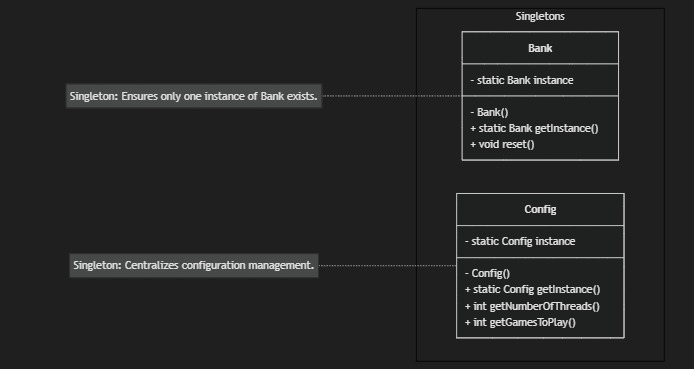
\includegraphics[width=0.9\textwidth]{singleton.jpg}
            \newline\footnotesize Singleton Pattern
            \vfill
        }
        \only<2>{
            \centering
            \vfill
            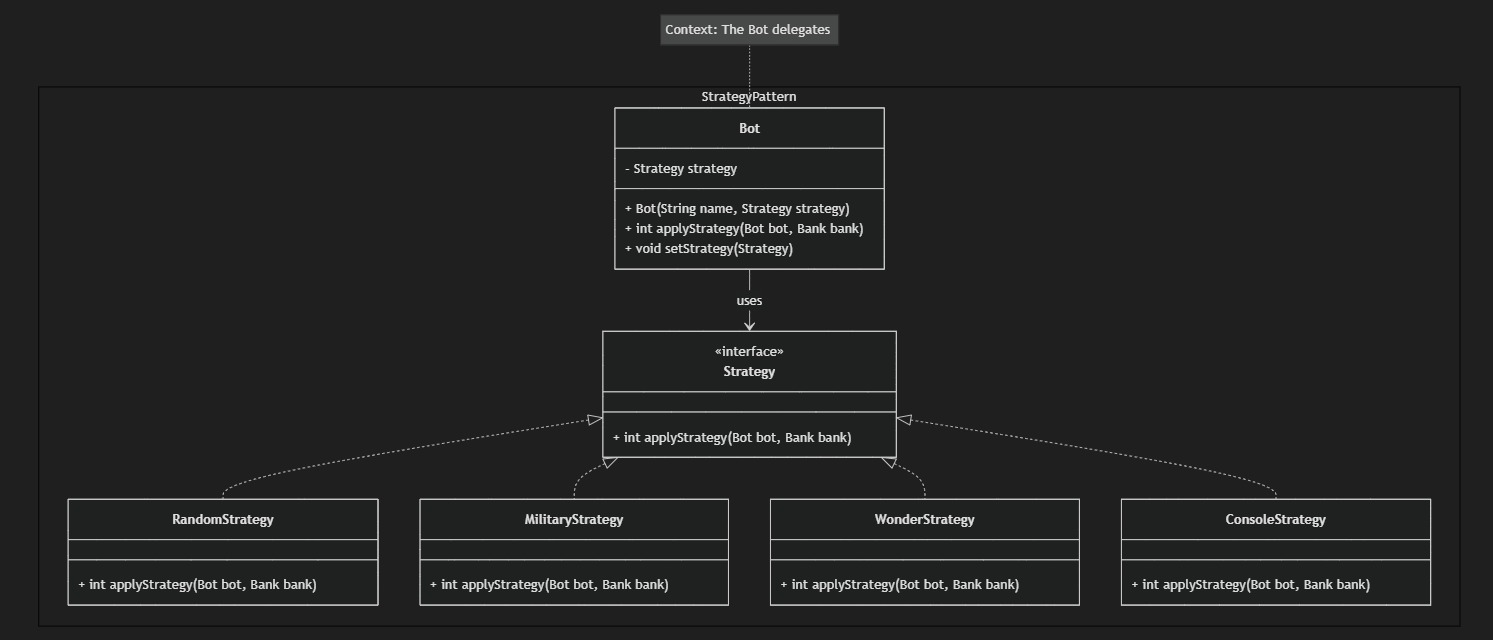
\includegraphics[width=0.9\textwidth]{strategty.jpg}
            \newline\footnotesize Strategy Pattern
            \vfill
        }
        \only<3>{
            \centering
            \vfill
            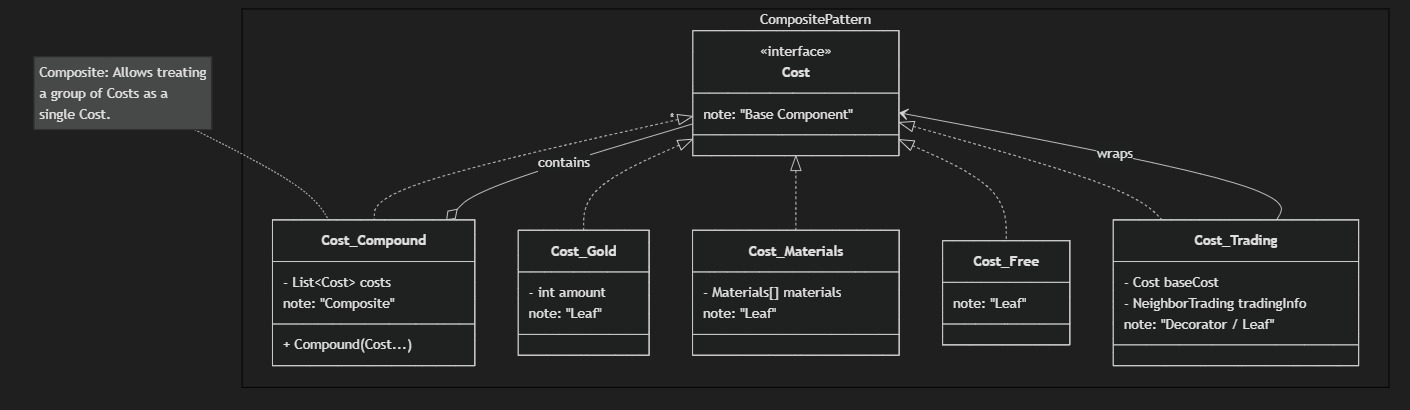
\includegraphics[width=0.9\textwidth]{composite.jpg}
            \newline\footnotesize Composite Pattern
            \vfill
        }
    \end{overlayarea}
    \end{block}
\end{frame}

\begin{frame}{Conception clé : Modélisation des effets de jeu}
    \begin{block}{Problématique}
        Comment représenter les 8 effets de jeu (victoire, ressources, actions spéciales...) de manière \textbf{flexible, sûre et maintenable} ?
    \end{block}

    \vspace{0.3cm}
    
    \begin{exampleblock}{Solution : Architecture modulaire avec Java moderne}
        \begin{columns}
            \begin{column}{0.45\textwidth}
                \begin{itemize}
                    \item \textbf{\texttt{sealed interface Effect}}
                    \begin{itemize}
                        \footnotesize
                        \item Définit tous les types d'effets possibles
                        \item Garantie de sécurité à la compilation
                    \end{itemize}
                    \item \textbf{Classes \texttt{record} immuables}
                    \begin{itemize}
                        \footnotesize
                        \item \texttt{Gold}, \texttt{Military}, \texttt{Science}...
                        \item Définition concise et sécurisée
                    \end{itemize}
                \end{itemize}
            \end{column}
            \begin{column}{0.55\textwidth}
                \begin{itemize}
                    \item \textbf{Méthode \texttt{apply(Player player)}}
                    \begin{itemize}
                        \footnotesize
                        \item Logique d'application spécifique
                        \item Cohésion forte, couplage faible
                    \end{itemize}
                    \item \textbf{Avantages}
                    \begin{itemize}
                        \footnotesize
                        \item Ajout/modification d'effets sans risque
                        \item Code clair et extensible
                    \end{itemize}
                \end{itemize}
            \end{column}
        \end{columns}
    \end{exampleblock}
\end{frame}

\section{Comment avons-nous organisé les tests ?}

\begin{frame}{Comment avons-nous organisé les tests ?}
  \begin{columns}
  \begin{column}{0.5\textwidth}
      \centering
      \vfill
      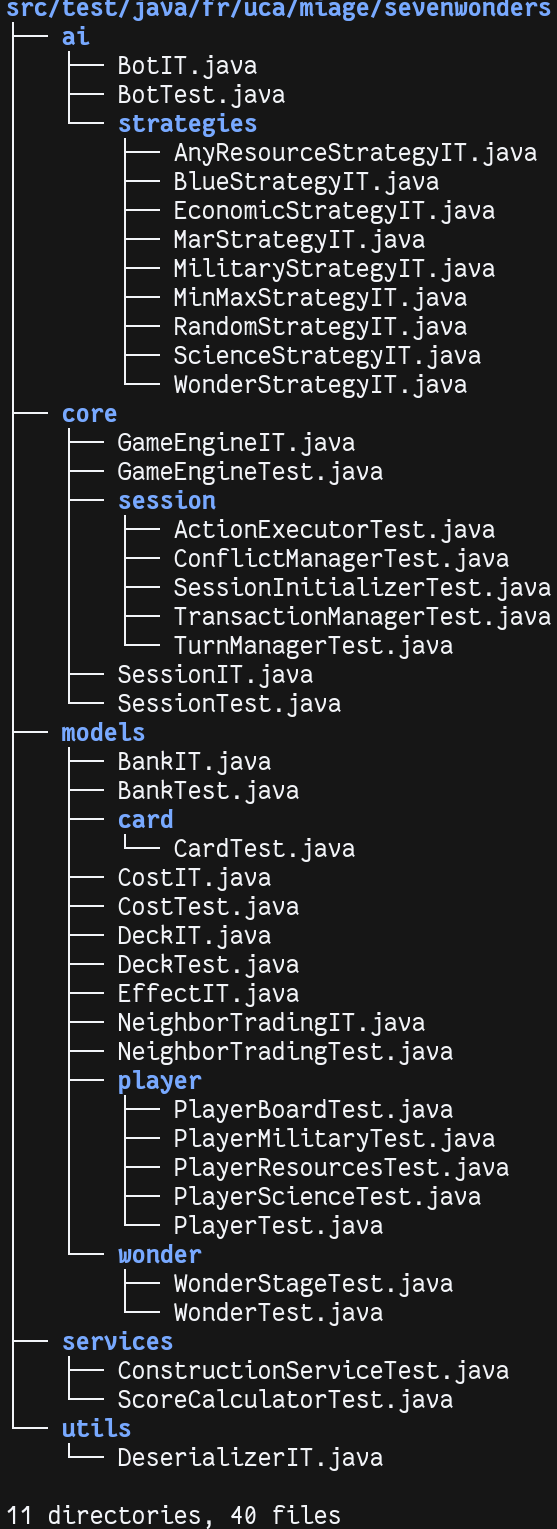
\includegraphics[height=\textheight -1cm]{tests.png}
  \end{column}

  \begin{column}{0.5\textwidth}
      \begin{block}{Stratégie de test : \newline }
          \textit{Tests unitaires (*Test.java) :}

          \begin{itemize}
              \item Couverture des composants critiques
              \item Isolation des fonctionnalités
          \end{itemize}

          \textit{Tests d'intégration (*IT.java) :}
          \begin{itemize}
              \item Validation des interactions
              \item Tests des interfaces
          \end{itemize}
      \end{block}
  \end{column}
  \end{columns}
\end{frame}

\section{Quels sont les points forts et les points faibles de notre implémentation ?}

\begin{frame}{Points forts et points faibles}
    \metroset{block=fill}
    \begin{columns}
        \begin{column}{0.5\textwidth}
            \begin{exampleblock}{Points forts}
                \begin{itemize}
                    \item \textbf{Documentation robuste} : Javadoc, commentaires, rapports détaillés et diagrammes UML.
                    \item \textbf{Expérience utilisateur} : Paramétrage fin du comportement du jeu via \texttt{config.toml}.
                    \item \textbf{Affichage} : Résultats sous forme de tableaux clairs et interface interactive attrayante.
                \end{itemize}
            \end{exampleblock}
        \end{column}

        \begin{column}{0.5\textwidth}
            \begin{alertblock}{Points faibles}
                \begin{itemize}
                    \item \textbf{Logs peu lisibles} : Structure peu claire et messages insuffisamment explicites.
  \item \textbf{Architecture monolithique} : Choix initial pour sa simplicité, mais limitant pour :
        \begin{itemize}
            \scriptsize
            \item[•] \textbf{Évolutivité} : Ajout de fonctionnalités plus complexe
            \item[•] \textbf{Maintenance} : Dépendances fortes entre composants
        \end{itemize}
            \item Utlisation de \textit{« valeures magiques »} pour les choix des robots et joueurs humains
                \end{itemize}
            \end{alertblock}
        \end{column}
    \end{columns}
\end{frame}

\section{Comment avons-nous géré le projet ?}

\begin{frame}{Comment avons-nous géré le projet ?}
    \begin{block}{Gestion du code source :}
        \vspace{0.5cm}\centering
    \vfill
    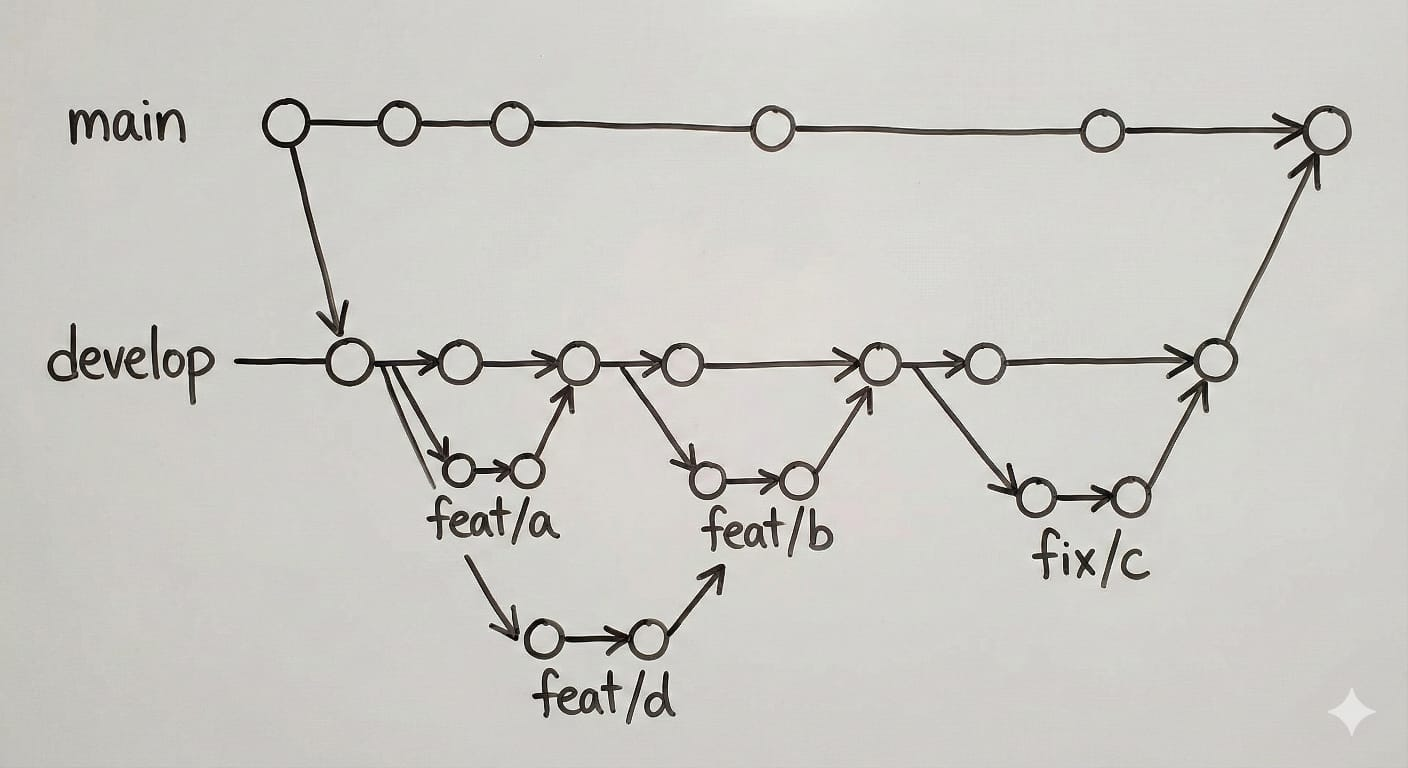
\includegraphics[width=0.9\textwidth]{branches.jpg}
    \newline\footnotesize Organisation des branches git
    \end{block}
\end{frame}

\begin{frame}{Comment avons-nous géré le projet ?}
    \begin{block}{Organisation du temps de travail :}
        \vspace{0.5cm}\centering
    \centering
    \vfill
    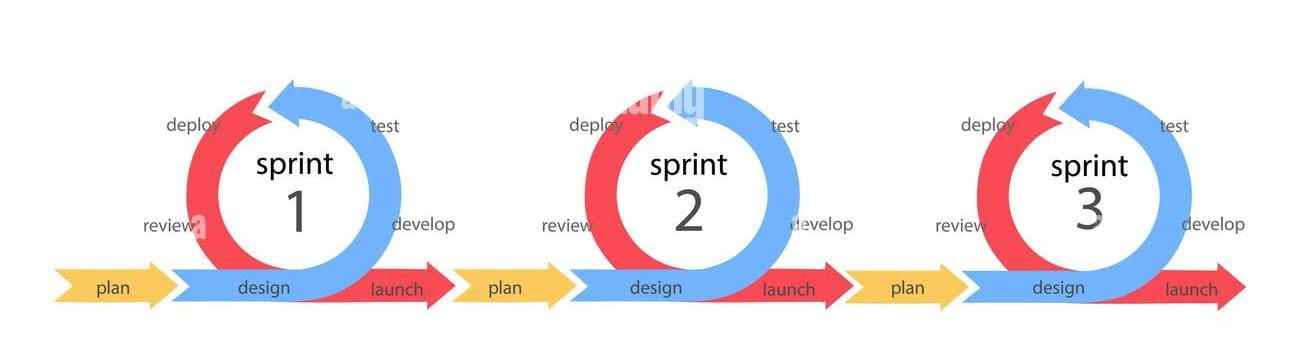
\includegraphics[width=0.9\textwidth]{sprints.jpg}
    \newline\footnotesize Division du travail en sprints aglies
    \end{block}
\end{frame}

\begin{frame}{Comment avons-nous géré le projet ?}
    \begin{alertblock}{Jalons non rélaisés :}
        \begin{itemize}
            \item Traduction du jeu \texttt{(i18n/l10n)}
            \item Passage de l'architecture monolithique vers des micro-services 
            \item Création d'un robot utilisant un \textit{LLM} pour sa prise de décisions
        \end{itemize}
    \end{alertblock}
\end{frame}

\section{Quelles inflexions ont éte prises en compte ?}

\begin{frame}{Quelles inflexions ont éte prises en compte ?}
    \begin{exampleblock}{Inflexions implémentées}
        \begin{itemize}
            \item \textbf{Inflexion 1 : Amélioration de la lisibilité} L'affiche utilise désormais des couleurs configurables par l'utilisateur dans la section \texttt{[colors]} du fichier \texttt{config.toml}.
            \item \textbf{Inflexion 2 : Lancement de parties en parallèle} Le nombre de threads est configurable via le paramètre \texttt{number\_of\_threads = 4} dans la configuration.
            \item \textbf{Inflexion 4 : Participation de l'utilisateur} L'utilisateur peut participer au jeu en activant l'option \texttt{enable\_real\_player = true} (ou \texttt{false} pour le mode automatique).
        \end{itemize}
    \end{exampleblock}

    \begin{alertblock}{Inflexion non implémentée}
        \begin{itemize}
            \item \textbf{Inflexion 3 : Mode duel} Cette fonctionnalité nécessitait des modifications trop importantes des règles de jeu et n'a pas pu être réalisée dans le délai imparti.
        \end{itemize}
    \end{alertblock}
\end{frame}

\begin{frame}[standout]
    \centering
    \Huge{Questions ?}

    \vspace{1cm}
    \large{Merci pour votre attention}
\end{frame}

\end{document}
